\classheader{2018-08-30}
\section*{Introduction to Probability (553.420) Review}
\subsection*{Part 1 - Counting}
\begin{enumerate}[label=\protect\circled{\arabic*}]
	\item Multiplication rule (Basic Counting Principle)
	\item Combinations/Permutations
	\begin{itemize}
		\item Sampling with or without replacement. $\Rightarrow$ Inclusion-Exclusion Principle
	\begin{equation*}
		\binom{n}{k} = \frac{n!}{k!(n-k)!} \qquad \qquad \Perm{n}{k} = \frac{n!}{(n-k)!}
	\end{equation*}
	\end{itemize}
	\item Birthday Problem
	\item Matching Problem (inclusion-exclusion principle)
	\begin{itemize}[label={--}]
		\item $P(A \cup B) = P(A) + P(B) - P(A \cap B)$
		\item $P(A \cup B \cup C) = P(A) + P(B) + P(C) - P(A \cap B) - P(A \cap C) - P(B \cap C) + P(A \cap B \cap C)$  
		\item etc...
	\end{itemize}
	\item $n$ balls going into $m$ boxes (all are distinguishable)
	\begin{example}
		$n$ balls numbered $1,2,\cdots, n$. $n$ boxes labelled $1,2,\cdots, n$. Distribute the balls into the boxes, one in each box. $M_i$ = ball $i$ is in box $i$
	\end{example}
	\item Multinomial Coefficients e.g. assign A, B, C, D, to different students $\rightarrow$ anagram problem\\ -- $n$ distinct objects into $r$ distinct groups
	\begin{equation*}
		\frac{n!}{n_1! n_2! n_3! \ldots n_r!} = \binom{n}{n_1, n_2, n_3, \ldots, n_r}
	\end{equation*}
	\item Pairing Problem
	\begin{equation*}
		2n \text{ people, paired up}
		\begin{cases}
			\text{ordered: } \binom {2n}{2,2,\cdots,2} \quad \text{e.g. different courts for players}\\\\
			\text{unordered: } \frac{\binom {2n}{2,2,\cdots,2}}{n!}
		\end{cases}
	\end{equation*}
	\item Partition of integers $\longrightarrow$ 
	$n$: sum of integer, \quad $r$: number of partitions 
	\begin{equation*}
		 \binom{n + r - 1}{r - 1} = \binom{n + r - 1}{n}
	\end{equation*}
\end{enumerate}
\subsection*{Basics of Probability}
\underline{Axioms}
\begin{enumerate}[label=\protect\circled{\arabic*}]
	\item $0 \leq P(A) \leq 1$, $\forall A$
	\item $P(\Omega) = 1 \rightarrow$ where $\Omega$ is the sample space
	\item Countable additivity
	\begin{itemize}
		\item if $A_1, \cdots, A_n$ are mutually exclusive, then
		\begin{equation*}
			P\bigg(\bigcup\limits_{i=1}^{\infty} A_i\bigg) = P(A_1) + P(A_2) + \cdots = \sum\limits_{i=1}^{\infty} P(A_i)
		\end{equation*}
	\end{itemize}
\end{enumerate}
$\Rightarrow P(A) = 1 - P(A^c)$\\
$P(A) = \mathlarger{\frac{|A|}{|\Omega|}}$
\subsubsection*{Conditional Probability}
\begin{equation*}
	P(A|B) = \mathlarger{\frac{P(A \cap B)}{P(B)}}	
\end{equation*}
\subsubsection*{Law of Total Probability}
\begin{equation*}
	P(A) = \sum\limits_j P(A|B_j) P(B_j) = \sum P(A \cap B_j) \quad \quad \underbrace{\bigcup\limits_j B_j = \Omega}_{\text{partition of $\Omega$}}
\end{equation*}
\subsubsection*{Bayes Rule}
\begin{equation*}
	P(B_i|A) = \mathlarger{\frac{P(A|B_i)P(B_i)}{\sum\limits_j P(A|B_j)P(B_j)}} \quad \quad \underbrace{\bigcup\limits_j B_j = \Omega}_{\text{partition of $\Omega$}}
\end{equation*}
\subsubsection*{Independent events}
If we have events $A_1, A_2, \cdots, A_n$, then
\begin{equation*}
	P(A_1 \cap A_2 \cap A_3 \cdots A_n) = P(A_1) \cdot P(A_2)\cdot P(A_3) \cdot \cdots P(A_n)
\end{equation*}
\subsection*{Introduction to Discrete and Continuous Random Variables}
\textbf{Random Variable} - a real valued function defined on the sample space of an experiment $X:\Omega \rightarrow \mathbb{R}$, $\forall \omega \in \Omega, X(\omega) \in \mathbb{R}$\\
\begin{tabularx}{\textwidth}{l|X|X}
 \textbf{Function} & \textbf{Discrete} & \textbf{Continuous} \\
\hline
\hline
Probability Function & PMF: $P(X=x)$ & PDF: $f_x(x)$\\
\hline
Probability Distribution & $\sum\limits_x P(X=x) = 1$ & $\int_x f_x(x) dx = 1$\\
\hline
Expectation & $E[X] = \sum\limits_x xP(X=x)$ & E[X] = $\int_x xf(x) dx$\\
\hline
Variance & $Var[X] = E[X^2] - (E[X])^2$ & $Var[X] = E[X^2] - (E[X])^2$
\end{tabularx}
\subsection*{Law of the Unconscious Statistician (LOTUS)}
1-dim $\quad E[g(x)] = \sum\limits_x g(x) P(X=x) \bigg/ E[g(x)] = \int_x g(x)f(x)dx$\\
2-dim $\quad E[g(X,Y)] = \sum\limits_y \sum\limits_x g(x,y) P(X=x,Y=y) \bigg/ E[g(X,Y)] = \int_y \int_x g(x,y) f(x,y)dx dy$
\subsection*{Discrete Distributions}
\begin{multicols}{2}
	\begin{enumerate}
	\item Bernoulli$(p)$
	\item Binomial$(n,p)$
	\item Poisson $(\lambda)$
	\item Geometric$(p)$
	\item Negative Binomial$(n,p)$
	\item Hypergeometric$(N,M,n)$
\end{enumerate}
\end{multicols}
\subsubsection*{Bernoulli Distribution}
$X$ is a random variable with Bernoulli$(p)$ distribution
\begin{tcolorbox}
\begin{gather*}
X \sim Bernoulli(p)\\
	P(X = x) = \begin{cases}
		p & x=1\\
		1-p & x = 0
	\end{cases}
\end{gather*}
\end{tcolorbox}
\subsubsection*{Binomial Distribution}
A sum of i.i.d. (identical, independent distribution) Bernoulli(p) R.V.
\begin{tcolorbox}
\begin{gather*}
	X \sim Binomial(n,p)\\ 
	\text{Support}: x \in \{0, 1, \cdots n\} \\
	n: \text{sample size}\qquad 
	p: \text{probability of success}\\
	P(X = k) = \binom{n}{k} p^k (1-p)^{(n-k)}\\
	E[X] = np \hspace{10em} Var(X) = np(1-p)
\end{gather*}
\end{tcolorbox}
\begin{itemize}
	\item Approximation methods $\Rightarrow$ 
	\begin{itemize}[label={--}]
		\item if $n$ is large, $p$ very small and $np < 10$. $\Rightarrow$ use Normal $(np, np(1-p))$
		\item $p \approx \frac{1}{2}$ $\Rightarrow$ Use Poisson $(\lambda = np)$
	\end{itemize}
	\item Mode: 
	\begin{itemize}[label={--}]
		\item if $(n+1)p$ integer, mode = (n+1)p or (n+1)p - 1.
		\item if $(n+1)p \notin \mathbb{Z}$ mode is $\left \lfloor{(n+1)p}\right \rfloor$
		\item \textbf{Proof:} consider $\mathlarger{\frac{P(X=x)}{P(X=x-1)}}$ going below 1.
	\end{itemize}
\end{itemize}
\subsubsection*{Poisson Distribution}
\begin{tcolorbox}
\begin{gather*}
	X \sim Poisson(\lambda)\\
	 x \in \{0, 1, \cdots \} \\
	\lambda : \text{parameter}\\
	P(X = x) = \frac{e^{-\lambda} \lambda^x}{x!}\\
	E[X] = \lambda \hspace{10em} Var(X) = \lambda
\end{gather*}	
\end{tcolorbox}
\textbf{Approximations}
\begin{itemize}
	\item if $n$ is large $\Longrightarrow$ Normal($\lambda,\lambda$)
\end{itemize}
\subsubsection*{Negative Binomial}
\begin{tcolorbox}
	\begin{gather*}
	X \backsim NB(r,p)\\
	\text{Support}: x = \{ r, r+1, \ldots \}\\
	r = \text{the rth success}\\
	p = \text{probability of success}\\
	P(X = k) = \binom{k + r-1}{k} \cdot (1-p)^r \cdot p^k
 	\end{gather*}
\end{tcolorbox}
A sum of i.i.d Geometric(p) R.V.\\
$\blacksquare$ $a^{th}$ head before $b^{th}$ tail
\begin{example}
	A coin has probability $p$ to land on a head, $q = 1-p$ to land on a tail.\\
	$P[5^{th} \text{tail occurs before the } 10^{th} \text{ head}]$?
	\begin{gather*}
	\begin{cases}
		= P[\text{5th tail occurs before or on the 14th flip}]\\
		= P[\text{Neg Binomial}(5,q) = 5,6,7,\cdots, 14]\\
		= \sum\limits_{x=5}^{14} \binom{x-1}{4} q^5 p^{x-5}
	\end{cases}	\text{(or)} \quad
	\begin{cases}
		= P[\text{at least 5 tails in 14 flips}]\\
		= P[binom(14,q) = 5,6,7,\cdots, 14]\\
		= \sum\limits_{x=5}^{14} \binom{14}{x} q^x p^{14-x}
	\end{cases}
	\end{gather*}
\end{example}
\subsubsection*{Geometric Distribution}
\begin{tcolorbox}
\begin{gather*}
	X \sim Geometric(p)\\
	\text{Support}: x \in \{1, 2, \cdots\}\\
	p: \text{probability of success}\\
	P(X = r) = (1-p)^{(r-1)} \cdot p\\
	\text{prob for 1st success on $r$th trial}\\
	E[X] = \frac{1}{p} \hspace{10em} Var(X) = \frac{1-p}{p^2}
\end{gather*}	
\end{tcolorbox}
\begin{example}
$\blacksquare$ Coupon Question\\
\underline{Variation A}: $N$ different types of coupons $\rightarrow P($ get a specific type$) = \frac{1}{N}$\\
\textit{Question:} $E[\text{draws to get 10 different coupons}]$?\\ 
\textit{Answer:}
\begin{gather*}
	X = X_1 + X_2 + \cdots + X_{10} \quad \quad \quad X_i = \text{\# draws to get the ith distinct coupon type}\\
	\boxed{X_i \backsim Geo(p_i)} \quad \quad p_i: \text{prob to get a new coupon $\leftarrow$ success, given that we have $i-1$ types of coupons}\\
	\text{Hence, } E[X_1] = 1\\
	E[X_2] = \frac{1}{p_2} = \frac{1}{\frac{N-1}{N}} = \frac{N}{N-1}\\
	E[X_3] = \frac{1}{p_3} = \frac{1}{\frac{N-2}{N}} = \frac{N}{N-2}\\
	\vdots\\
	E[X_{10}] = \frac{1}{p_{10}} = \frac{1}{\frac{N-9}{N}} = \frac{N}{N-9}\\
	\text{So, } \quad E[X] = E[X_1] + E[X_2] + \cdots + E[X_{10}] = E[\sum\limits_{i=1}^{10} X_i] = 1 + \frac{N}{N-1} + \frac{N}{N-2} + \cdots + \frac{N}{N-9}
\end{gather*}
\underline{Variation B}: Same setting, now you draw 10 times.\\
\textit{Question:} $E[\#$ different types of coupons$]$?\\ 
\textit{Answer:}
\begin{gather*}
	X = I_1 + I_2 + \cdots + I_N\\
	I_i
	\begin{cases}
		1 & \text{if we have this type of coupon}\\
		0 & \text{o/w}
	\end{cases}\\
	\begin{align*}
		E[I_i]  & = P(\text{we draw coupon i in 10 draws})\\
		& = 1 - P(\text{we don't have coupon i}) \quad \quad \quad \text{we use binomial distribution where } 1-P(N=0)\\
		& = 1 - \bigg( \frac{N-1}{N} \bigg)^{10}
	\end{align*}\\
	E[X] = E[\sum\limits_{i=1}^{N} I_i] = N E[I_i] = \boxed{N \bigg[ 1 - \bigg( \frac{N-1}{N} \bigg)^{10} \bigg]}
\end{gather*}
\end{example}
\subsubsection*{Hypergeometric Distribution}
\begin{tcolorbox}
	\begin{gather*}
		X \sim Hyp(N, M, n)\\
		N \in \{0, 1, 2, \ldots \} \quad M \in \{0, 1, \ldots, N\} \quad n \in \{0, 1, \ldots, N\}\\
		\text{Support}: k \in \{\max(0, n + M - N), min(n, M)\}\\
		N \quad \text{is the population size}\qquad
		K \quad\text{is the no. of success states in the population}\\
		n \quad\text{is the no. of draws (i.e. quantity drawn in each trial)}\\
		k \quad\text{is the no. of observed successes}\\
		P(X = k) = \frac{\binom{M}{k} \binom{N - M}{M - k - 1}}{\binom{N}{n}}
	\end{gather*}
\end{tcolorbox}
\subsection*{Continuous Distributions}
\subsubsection*{Uniform Distribution}
\begin{tcolorbox}
	\begin{gather*}
		X \sim Unif(a,b)\\
		f_X(x) = 
		\begin{cases}
			\frac{1}{b-a} & a \leq x \leq b\\
			0 & o/w
		\end{cases}\\
		E[X] = \frac{a + b}{2} \hspace{10em} Var(X) = \frac{(b-a)^2}{12}
	\end{gather*}
\end{tcolorbox}
\subsubsection*{Normal Distribution}
\begin{tcolorbox}
	\begin{gather*}
	X \backsim N(\mu, \sigma^2) \Rightarrow Z = \frac{X- \mu}{\sigma} \backsim N(0,1) \text{ with CDF } P(Z \leq z) = \Phi(z)\\
	\Phi(-x) = 1 - \Phi(x) \\
	\text{Support:} \quad x \in (-\infty, \infty)\\
	f_X(x) = \frac{1}{\sqrt{2\pi} \sigma}e^{\frac{-(x - \mu)^2}{2\sigma^2}}\\
	E[X] = \mu \hspace{10em} Var(X) = \sigma^2
\end{gather*}
\end{tcolorbox}
\subsubsection*{Exponential distribution}
\begin{tcolorbox}
\begin{gather*}
	X \sim Exp(\lambda)\\
	\text{Support:} \quad x \in [0, \infty)\\
	f_X(x) = \lambda e^{-\lambda x}\\
	E[X] = \frac{1}{\lambda} \hspace{10em} Var(X) = \frac{1}{\lambda^2}
\end{gather*}	
\end{tcolorbox}

\textbf{Lack of memory property:} $P(X \geq s+t | X\geq t) = P(X \geq s)$
\begin{itemize}
	\item $M$ = min of $exp(\lambda)$ and $exp(\mu) \Rightarrow M \backsim exp(\lambda + \mu)$
	\item $M$ = min of $X_1, X_2, \cdots, X_n$, where $X_i \backsim_{\text{\tiny i.i.d.}} exp(\lambda) \Rightarrow exp(n\lambda)$ 
\end{itemize}
\subsubsection*{Gamma Distribution}
\begin{tcolorbox}
	\begin{gather*}
		X \sim Gamma(\alpha, \beta)\\
		\text{Support:} \quad x \in [0, \infty)\\
		F_X(x) = \frac{\beta^\alpha}{\Gamma(\alpha)} x^{\alpha - 1} e^{-\beta x}\\
		E[X] = \frac{\alpha}{\beta} \hspace{10em} Var(X) = \frac{\alpha}{\beta^2}\\
		\textbf{Gamma Function:} \quad \Gamma(z) = (z - 1)! = \int_0^\infty x^{z-1} e^{-x} dx\\
	\end{gather*}
\end{tcolorbox}
\subsubsection*{Beta Distribution}
\begin{tcolorbox}
\begin{gather*}
	X \sim Beta(\alpha, \beta)\\
	\text{Support:} \quad x \in [0, 1]\\
	f_X(x) = \frac{\Gamma(\alpha + \beta)}{\Gamma(\alpha) \Gamma(\beta)} x^{\alpha - 1} (1 - x)^{\beta - 1}\\
	E[X] = \frac{\alpha}{\alpha + \beta} \hspace{10em} Var(X) = \frac{\alpha \beta}{(\alpha + \beta)^2(\alpha + \beta + 1)}
\end{gather*}	
\end{tcolorbox}

\subsubsection*{Chi-Square}
\begin{gather*}
	\textbf{Chi-Square: } \chi^2_n \text{is Chi-square with degrees of Freedom }n\\
	\chi^2_n = Z_1^2 + Z_2^2 + \cdots + Z_n^2 \quad \quad \text{where $Z_i \backsim$ standard normal}. Z_i \backsim Gamma\bigg(\frac{1}{2},\frac{1}{2}\bigg)\\
	\Rightarrow \chi^2_n = n \text{ i.i.d. } Z_i \backsim Gamma\bigg(\frac{1}{2},\frac{1}{2}\bigg)\\
	= Gamma\bigg(\frac{n}{2},\frac{1}{2}\bigg)
\end{gather*}
\subsection*{CDF in General}
\begin{itemize}
	\item $F_x(t) = P(X \leq t)$
	\begin{align*}
		& = \sum\limits_{x \leq t} P(X = x) \quad \quad \text{discrete}\\
		& = \int_{-\infty}^{t} f(x) dx \quad \quad \quad \text{continuous}
	\end{align*}
	\item \textbf{Discrete: } "Left open, right closed" $\Rightarrow$ if you flip the sign (from $<$ to $\leq$) in the left, you flip the sign of $a$ (from $a$ to $a^-$)
	\begin{itemize}[label={--}]
		\item $P(a < x \leq b) = F(b) - F(a)$
		\item $P(a \leq x \leq b) = F(b) - F(a^-)$
		\item $P(a < x < b) = F(b^-) - F(a)$
		\item $P(a \leq x < b) = F(b^-) - F(a^-)$
	\end{itemize}
	\item \textbf{Continuous: } (because a point doesn't have a mass)
	\begin{equation*}
		P(a \leq x \leq B) = \int_a^b f(x) dx = F(b) - F(a)
	\end{equation*}
\end{itemize}
\subsection*{Density Transformation}
For density transformation \textbf{e.g.} finding pdf of $U = X + Y$
\begin{multicols}{2}
	\begin{itemize}[label={--}]
	\item Convolution
	\item MGF
	\item Jacobian
	\item CDF Transformation
\end{itemize}
\end{multicols}
\begin{itemize}
	\item Use CDF: Computer $P(Y \leq y) = P(g(x) = y)$
	\item \textbf{1-dim: } If Y is monotonically increasing or decreasing: $Y = g(x) \quad \boxed{f_Y(y) = f_X(x(y)) \cdot |(x^{-1})'(y)|}$
	\item \textbf{2-dim: } Joint Density:
	\begin{gather*}
		(X, Y) \rightarrow (U, V) \quad \quad \quad U = h_1(X, Y) \quad \quad V = h_2(X,Y)\\
		f_{U,V}(u,v) = f_{X,Y}(x(u,v), y(u,v)) \cdot |J|\\
		\text{where } \quad J = \begin{vmatrix}
			\dfrac{\partial x}{\partial u} & \dfrac{\partial x}{\partial v}\\\\
			\dfrac{\partial y}{\partial u} & \dfrac{\partial y}{\partial v}
		\end{vmatrix} \quad \text{ determinant}
	\end{gather*}
	\item if $Z = X + Y\quad$ (2-dim $\rightarrow$ 1-dim) use CDF. Compute $P(Z \leq z) = P(X+Y \leq z)$. Integrate $f(x,y)$ over this region.
\end{itemize}
\subsection*{Joint Distribution}
\begin{equation*}
	\begin{split}
		& \textbf{Discrete}\\
		P_{X,Y}(x,y) = & P(X=x, Y=y)\\
		\text{Indep} \Rightarrow & P_X(x)P_Y(y)
	\end{split}\quad \quad
	\begin{split}
		& \textbf{Continuous}\\
		F_{X,Y}(x,y) & = f_X(x) f_Y(y)\\
		& = \dfrac{\partial^2}{\partial x \partial y} F_{X,Y}(x,y)
	\end{split}
\end{equation*}
\begin{itemize}
	\item \textbf{Marginal Density/PMF}:
	\begin{gather*}
		\textbf{Continuous: }\quad \quad f_X(x) = \int_x f_{X,Y}(x,y)dy \quad \textit{and} \quad f_Y(y) = \int_y f_{X,Y}(x,y)dx\\
		\textit{* the bounds for y in the integration can depend on x, and vice versa}\\
		\textbf{Discrete: }\quad \quad P_X(x) = \sum\limits_y P(X=x,Y=y) \quad \textit{and} \quad P_Y(y) = \sum\limits_x P(X=x,Y=y) 
	\end{gather*}
	\item Use joint pdf to compute probability
	\begin{center}
		e.g. $P(X < Y) = \int\limits_0^\infty \int\limits_x^\infty f(x,y)dy dx \quad \quad \quad$ assume $x>0, y>0$\\
		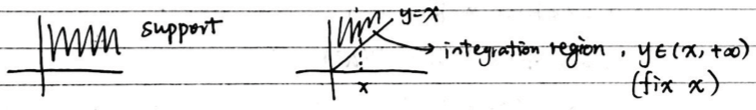
\includegraphics{0-1}
	\end{center}
	\item \textbf{Independence: } If $X,Y$ are independent, then 
	\begin{gather*}
		\textbf{Continuous: }\quad \quad f(x,y) = f_X(x)f_Y(y)\\
		\textbf{Discrete: }\quad \quad P(X=x, Y=y) = P(X=x) P(Y=y)
	\end{gather*}
	\item \textbf{Convolution: } assume $X,Y$ are independent
	\begin{gather*}
		\textbf{Discrete: }\quad \quad P_{X+Y}(a) = \sum\limits_y P_X(a-y)P_Y(y) = \sum\limits_x P_X(x)P_Y(a-x)\\
		\textbf{Continuous: }\quad \quad f_{X+Y}(a) = \int_y f_X(a-y)f_Y(y)dy = \int_y f_X(x)f_Y(a-x)dx\\
		\textbf{MGF: }\text{we can use this} \quad \quad M_{X+Y}(t) = M_X(t) M_Y(t) \longrightarrow \text{then identify dist of X+Y from mgf} 
	\end{gather*}
\end{itemize}
\subsection*{Conditional distribution}
\begin{align*}
	\textbf{Discrete} \quad \quad
	& P_{X|Y=y}(x|y) = \frac{P_{X,Y}(x,y)}{P_Y(y)} = \frac{P(X=x, Y=y)}{P(Y=y)}\\
  & \Rightarrow \sum\limits_y P_{X,Y}(x,y) = \sum\limits_y P_{X|Y=y}(x|y) \cdot P_Y(y)\\
  \textbf{Continuous} \quad \quad & f_{X|Y=y}(x|y) = \frac{f_{X,Y}(x,y)}{f_Y(y)}\\
  & \Rightarrow f_X(x) = \int_y f(x,y)dy = \int_y f_{X|Y=y}(x|y)\cdot f_Y(y)dy
\end{align*}
\subsubsection*{Conditional Expectation}
\begin{align*}
	& E[X|Y=y] = \int_x xf(x|y) dx\\
	& E[X|Y]: \text{compute } E[X|Y=y] \text{ first, replace $y$ with $Y$}
\end{align*}
\subsection*{Ordered Statistics}
Consider $X_1, X_2, \cdots, X_n \quad \quad X_{(j)}$ = j-th smallest
\begin{align*}
	F_{\max(X_i)}(t) & = P(\max X_i \leq t) = P(X_1 \leq t)\cdot P(X_2 \leq t) \cdots P(X_n \leq t)\\
	& = [F_X(t)]^n \quad \quad \quad
	\boxed{f_{\max X_i}(t) = nF(t)^{n-1} f_X(t)}\\
	 F_{\min(X_i)}(t) & = 1 - P(\min x_i \geq t) = 1-P(X_1 \geq t)\cdot P(X_2 \geq t) \cdots P(X_n \geq t)\\
	 & = 1 - [1 - F_X(t)]^n \quad \quad \quad \boxed{f_{\min X_i}(t) = n[1 - F(t)]^{n-1} f_X(t)}
\end{align*}
\textbf{General:} $j$-th order statistic
\begin{equation*}
	f_{x(j)}(t) = \binom{n}{j-1,1,n-j} F_X(t)^{j-1}\cdot f_X(t) \cdot [1-F_X(t)]^{n-j}
\end{equation*}
\subsection*{Expectation and Variance}
\begin{gather*}
	\textbf{Law of Total Expectation: } E[X] = E[E[X|Y]]\\
\textbf{Law of Total Variance: } Var(X) = E[Var(X|Y)] + Var[E(X|Y)]
\end{gather*}
\subsubsection*{Expectation}
\begin{enumerate}[label=\protect\circled{\arabic*}]
	\item linearity of expectation
	\item How to compute
	\begin{enumerate}
		\item LOTUS or definition (use density to integrate)
		\item MGF: $M^{(n)}(0) = E[X^n]$ or by recognition
		\item $E[X^2] = Var[X] + E[X]^2$
		\item Tail probability X is non-neg R.V. $(x>0)$ then $E[X] = \sum\limits_{t=0}^\infty P(X \geq t)$ \textit{or} $= \int\limits_0^\infty P(X \geq t) dt$
	\end{enumerate}
\end{enumerate}
\subsubsection*{Variance}
\begin{enumerate}[label=\protect\circled{\arabic*}]
	\item $Var(X_1 + X_2 + \cdots + X_n) = \sum\limits_{i=1}^n Var(X_i) + \sum\limits_{i \neq j} Cov(X_i, X_j)$
	\begin{center}
		if $X_i, X_j$ identical (not independent) $ = n Var(X_i) + n(n-1)Cov(X_i, X_j) \quad \quad i\neq j$
	\end{center}
	\item \textbf{Covariance: }
	\begin{align*}
		Cov(X,Y) & = E[XY] - E[X]E[Y]\\
		Cov(X,c) & = 0 \quad \quad c \textit{ is a constant}\\
		Cov(X+Y,Z) & = Cov(X,Z) + Cov(Y,Z)\\
		Cov(cX,dZ) & = cd \cdot Cov(X,Z) 
	\end{align*}
	\item \textbf{Correlation Coefficient:}
	\begin{equation*}
		\rho(X,Y) = \frac{Cov(X,Y)}{\sqrt{Var(X) Var(Y)}} = \frac{Cov(X,Y)}{\sigma_x \sigma_y}
	\end{equation*}
\end{enumerate}
\subsection*{Limit Theorems}
\subsubsection*{Markov's Inequality}
For any non-negative random variable $X$
\begin{equation*}
	P(X \geq a) \leq \frac{E(X)}{a} \tag{for \underline{any} $a > 0$}
\end{equation*}
\begin{proof}
	Let $X \geq 0$ a random variable and let $a > 0$.
	Define new random variable from $X$ as $Y_a$
	\begin{gather*}
		Y_a =
		\begin{cases}
 		0 & \text{if }	X < a\\
 		a & \text{if }	X \geq a\\
		 \end{cases}\\
		0 \leq Y_a \leq X \Longrightarrow \underbrace{E[Y_a]}_{a\cdot P(X \geq a)} \leq E[X]\\
		E[Y_a] = 0 \cdot P(Y_a < a) + a\cdot P(X \geq a)\\
		 E[Y_a] = a\cdot P(X \geq a) \leq E[X] \Longrightarrow \boxed{P(X \geq a) \leq \frac{E(X)}{a}}
	\end{gather*}
\end{proof}
\subsubsection*{Chebyshev's Inequality}
For any random variable Y with mean $\mu_y$ and variance $\sigma_y^2$
\begin{equation*}
	P(|Y - \mu)y| \geq c) \leq \frac{\sigma_y^2}{c^2} \tag{for \underline{any} $c > 0$}
\end{equation*}
\begin{proof}
	\begin{gather*}
		P(|Y - \mu_y)| \geq c) = P(\underbrace{|Y - \mu_y)|^2}_{=X} \geq c^2)\\
		P(|Y - \mu_y)|^2 \geq c^2) \leq \frac{E[|Y - \mu_y|^2]}{c^2} = \frac{\sigma_y^2}{c^2}
	\end{gather*}
\end{proof}
This is the same as
\begin{itemize}[label={--}]
	\item $P(|Y - \mu_y| \geq k \sigma_y) \leq \frac{1}{k^2}$
	\item $P(|Y - \mu_y| \leq k \sigma_y) \geq \underbrace{1- \frac{1}{k^2}}_{\text{very conservative}}$
\end{itemize}
\subsubsection*{Weak Law of Large Numbers}
If $X_1, X_2, \cdots$ are $i.i.d.$ with a mean $\mu$
\begin{equation*}
	\text{then} \qquad \mathlarger{\mathlarger{\Lim{n \rightarrow \infty}}} {\large P}\bigg( \bigg| \frac{X_1 + X_2 + \cdots + X_n}{n} - \mu \bigg| \geq \epsilon \bigg) = 0
\end{equation*}